% TO COMPILE %

%%%%%%%%%%                             %%%%%%%%%%
%%%%%%%%%% AUTO INSERTION D'UNE ENTETE %%%%%%%%%%
%%%%%%%%%%                             %%%%%%%%%%
%%%%%%%%%%     POUR UN FICHIER TEX     %%%%%%%%%%
%%%%%%%%%%                             %%%%%%%%%%

%%%%%%          %%%%%%
%%%%%% PACKAGES %%%%%%
%%%%%%          %%%%%%

\documentclass[a4paper]{article}
\usepackage{fullpage}
\usepackage[utf8]{inputenc}
\usepackage[francais]{babel}
\usepackage{graphicx}
\usepackage{listings}
\usepackage{color} 
\usepackage{enumerate}
\usepackage{amsfonts}
\usepackage{amssymb}
\usepackage{amsmath}
\usepackage{wasysym}
\usepackage{chemarrow}
\usepackage[colorlinks=true, urlcolor=blue]{hyperref}

%%%%%%              %%%%%%
%%%%%% MISE EN PAGE %%%%%%
%%%%%%              %%%%%%


%%%%% Marges %%%%%
%\addtolength{\textwidth}{3cm}
\addtolength{\oddsidemargin}{-1.3cm}
\textheight=24cm % longueur utile de la page
\topmargin=-1cm % marge haute
%\bottommargin=-1cm % marge haute
\headsep=20pt % séparation 20 points entre entête et texte
%\footskip=30pt % idem séparation pied de page
\addtolength{\footskip}{20pt}
%%%%% Entetes et Enpieds de pages %%%%%
\usepackage{fancyhdr}
\pagestyle{fancy}
\lhead{\footnotesize{\textit{Ludovic Brochard, Fabien Kuntz, Benoît Védrenne}}}
\rhead{\footnotesize{\textit{Projet Algorithmes du Monde Réel}}}

%%%%% Numérotation sections %%%%
\setcounter{secnumdepth}{3}
\setcounter{tocdepth}{3}

%%%%% Types enumerate %%%%%
\let\enumeratesav\enumerate
\let\endenumeratesav\endenumerate

\renewenvironment{enumerate}{
\enumeratesav
 \setlength{\itemsep}{0.5pt}
 \setlength{\parskip}{0pt}
 \setlength{\parsep}{0pt}}
\endenumeratesav

\renewcommand{\labelenumi}{-}
\renewcommand{\labelenumii}{$\bullet$}
\renewcommand{\labelenumiii}{$\star$}
\renewcommand{\labelenumiv}{\_}

%%%%% Titre %%%%%
\newlength{\larg}
\setlength{\larg}{14.5cm}

%%%Zone de Code%%%
\definecolor{gray}{gray}{0.86}  

\lstset{numbers=left, tabsize=2, frame=single, breaklines=true,
basicstyle=\ttfamily,numberstyle=\tiny\ttfamily, framexleftmargin=13mm,
backgroundcolor=\color{gray}, xleftmargin=14mm} 

\newsavebox{\fmbox}
\newenvironment{fmpage}[1]{\begin{lrbox}{\fmbox}\begin{minipage}{#1}}{\end{minipage}\end{lrbox}\fbox{\usebox{\fmbox}}}


%%%%%%          %%%%%%
%%%%%% DOCUMENT %%%%%%
%%%%%%          %%%%%%


\begin{document}


%%%%% Page de présentation %%%%%
\thispagestyle{empty}

\setlength{\unitlength}{1in}

%%%%% Image de fond %%%%%
% \begin{picture}(0,0)
% \put(0.2,-7){\includegraphics[width=\textwidth]{images/bx1_trans.eps}}
% \end{picture}

\begin{flushright}
 \noindent {\rule{\larg}{0.5mm}}
\end{flushright}
\vspace{7mm}
\begin{flushright}
 \Huge{\bf Algorithmes du Monde Réel} \\
 \Huge{\bf Projet} \\
 ~\\
 \huge{Partie 1 - Réductions}\\
 % \Large{\bf{\emph{Fabien Kuntz}}}
\end{flushright}
\vspace{7mm}
\begin{flushright}
 {\rule{\larg}{0.5mm}}
\end{flushright}
\vspace{2mm}
\begin{flushright}
 \large{\bf Professeurs : M. Zeitoun, A. Muscholl, C. Gavoille} \\
 ~\\
 \large{Master 2 Informatique}\\
 ~\\
 % \today
 \vspace{10cm}
 \large{Ludovic Brochard, Fabien Kuntz, Benoît Védrenne}
{\rule{\larg}{0.5mm}}
\end{flushright}

\newpage

\addtolength{\oddsidemargin}{1cm}

%%%%% Table des matières %%%%%
\thispagestyle{empty}
\tableofcontents
\newpage

\setcounter{page}{1}


%%%%%%              %%%%%%
%%%%%% ZONE DE CODE %%%%%%
%%%%%%              %%%%%%

 %==============================================================================
 \begin{frame}
  \frametitle{Le projet}
  
  \begin{block}{Principe}
   \begin{itemize}
    \item Deux robots : Maître et Esclave
	  \uncover<2->{
    \item Robot Maître : capteurs et moteurs}
	  \uncover<3->{
    \item Robot Esclave : seulement moteurs}
	  \uncover<4->{
    \item Maître communique les ordres à l'Esclave par Bluetooth}
	  \uncover<5->{
    \item Esclave : pas de décision}
   \end{itemize}
  \end{block}

  \uncover<6->{
  \begin{block}{But}
   \begin{itemize}
    \item Accomplir une mission non triviale mettant en jeu les deux robots
	  \uncover<7->{
    \item Vérifier cette mission en modélisant en Altarica}
    \uncover<8->{
    \item Etudier la possibilité d'une generation de code automatique}
   \end{itemize}
  \end{block}
  }

 \end{frame}

 \section{Choix}
 Dans cette partie, nous allons présenter quelques uns des choix que
 nous avons faits concernant notre programme.

  \subsection{Langage}
  Nous avions le choix de faire ce projet en \emph{C} ou en
  \emph{C++}. Nous avons choisi \emph{C++} pour la simple raison que des
  structures de données intéressantes (notamment \emph{vector}) sont
  déjà présentes dans ce langage alors qu'elles ne le sont pas dans le
  langage \emph{C}.
  
  \subsection{Structure de données}
  Dans ce projet, nous avions à faire le choix d'une structure de
  données pour représenter les graphes. Nous avons suivi les conseils en
  décidant d'utiliser des listes d'adjacence.

  Plusieurs raisons nous ont poussés à utiliser les listes d'adjacence
  plutôt que d'autres structures\footnote{Il n'y a ici, pas de bon choix
  à proprement parler, le mieux serait de faire au cas par cas (nous en
  parlerons dans le bilan du rapport).} :
  \begin{enumerate}
   \item La liste d'adjacence est une des structures qui prend le moins
	 de place en mémoire car elle ne stocke que les sommets voisins
	 (contrairement à une matrice d'adjacence par exemple).
   \item La liste d'adjacence est très efficace lorsqu'on a à
	 considérer la liste des voisins des sommets (c'est son essence
	 même), ce qui est le cas pour nos réductions.
   \item La liste d'adjacence est évidemment plus efficace que n'importe
	 quelle structure d'incidence lorsqu'il s'agit de considérer les
	 sommets plutôt que les arêtes.
  \end{enumerate}

    \subsection{Dépendances et Relations}
  Le programme est simple d'utilisation puisqu'il suffit de le lancer
  avec un fichier d'entrée de type graphe issu du programme
  \emph{gengraph} de
  \emph{C. Gavoille}\footnote{\url{http://dept-info.labri.fr/~gavoille/gengraph.c}}
  ainsi qu'avec le numéro du problème et éventuellement des paramètres
  propres au problème.\\
  Le programme se déroule de la manière suivante :
  \begin{enumerate}
   \item Le fichier de graphe est lu à partir du fichier de graphe
	 fourni. 
   \item Selon le problème sélectionné, on lance la réduction
	 correspondante. 
   \item Une formulation en clauses de type \emph{CNF} est créée et
	 envoyée au \emph{SATSolver} \emph{Minisat}. 
   \item \emph{Minisat} crée une solution (si cela est possible).
   \item La solution fournie est analysée afin de pouvoir être
	 traitée. De cette manière, nous connaissons la solution au
	 problème voulu sur le graphe passé en paramètre. 
  \end{enumerate}
  
  En décrivant l'exécution du programme de cette façon, il est aisé de
  voir apparaître les relations entre les modules de notre programme.

  La fonction principale \emph{main}, contenue dans \emph{Solve.cpp},
  joue le rôle du tri des arguments et de construction du
  graphe. Ensuite, est appelée la réduction voulue, contenue dans les
  fichiers portant le nom d'un problème (ou leur abréviation). Une fois
  la réduction effectuée par ce fichier, celui-ci appelle un ``parser''
  pour \emph{Minisat} (dans \emph{MinisatBuilder.cpp}) qui gère le fait
  d'écrire un fichier d'entrée à \emph{Minisat}, de lancer le
  \emph{SAT-Solver} et d'analyser sa sortie. Une fois la sortie
  analysée, une assignation des variables est donnée. Celle-ci nous
  permet alors de fournir l'ensemble des arêtes ou sommets nécessaire
  définissant une solution du problème donné sur le graphe donné.\\

  Voici un graphe représentant simplement les relations entre les
  différentes parties du programme (fig.\ref{grapheExec} page
  \pageref{grapheExec}).
  \begin{figure}[!ht]
   \begin{center}
    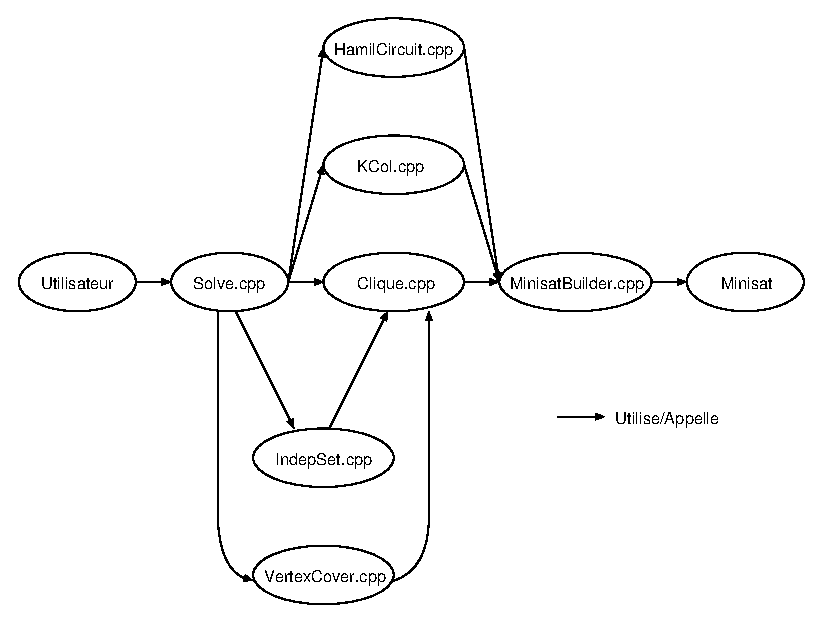
\includegraphics{images/grapheExec.eps}
    \caption{Relations entre les différentes parties du
    programme\label{grapheExec}}
   \end{center}
  \end{figure}

  \subsection{Extension des fichiers}
  Étant donné que nous générons des fichiers avec notre programme, nous
  avons aussi choisi des noms et extensions différentes selon le but du
  fichier.

  En effet nous avons introduit trois extensions différentes :
  \begin{enumerate}
   \item \emph{graph.gin} $\leadsto$ Fichier graphe de type
	 \emph{gengraph} passé en paramètre par l'utilisateur au
	 programme
   \item \emph{graph.sat} $\leadsto$ Fichier qui contient la formule de
	 type \emph{CNF\footnote{Conjunctive Normal Form}} générée par
	 notre programme à partir du choix du problème et du graphe.
   \item \emph{graph.sol} $\leadsto$ Fichier qui contient la solution
	 retournée par \emph{minisat}.
  \end{enumerate}

  Nous avons fait le choix de laisser ces fichiers sur le disque après
  exécution du programme, dans le cas où l'utilisateur souhaiterait y
  jeter un \oe{}il\footnote{Les utilisateurs que nous sommes ont
  beaucoup apprécié cette possibilité.}.

 \section{Idées des réductions}
 Nous allons dans cette partie vous présenter très brièvement les idées
 de réductions que nous avons utilisées. Nous allons seulement citer les
 quelques propriétés caractérisant nos problèmes qui nous ont permis de
 générer les formules \emph{CNF}.
 
 Nous citerons aussi ce que nous avons appelé les ``cas
 faciles'', c'est à dire les cas où nous n'avons pas besoin de
 \emph{Minisat} pour répondre à nos problèmes (problème de décision).

  \subsection{\emph{K-Col} $\leq_P$ \emph{SAT}}
  \underline{Propriétés caractérisant \emph{K-Col} :}
  \begin{enumerate}
   \item Chaque sommet est colorié.
   \item Il n'y a qu'une seule couleur par sommet.
   \item Deux sommets qui se suivent n'ont pas la même couleur.
  \end{enumerate}

  \underline{Cas faciles :}
  \begin{enumerate}
   \item Le nombre de couleurs est négatif.
   \item Le nombre de couleurs est supérieur au nombre de sommets.
  \end{enumerate}

  \subsection{\emph{Circuit Hamiltonien} $\leq_P$ \emph{SAT}}
  \underline{Propriétés caractérisant \emph{Circuit Hamiltonien} :}
  \begin{enumerate}
   \item Chaque noeud est dans le circuit.
   \item Un noeud a exactement une position dans le circuit sauf pour le
	 premier/dernier.
   \item Deux sommets non voisins ne peuvent pas se suivre dans le
	 circuit.
   \item Deux sommets n'ont pas la même position dans le circuit.
   \item Le dernier sommet du circuit doit aussi être le premier.
  \end{enumerate}

  \underline{Cas faciles :}
  \begin{enumerate}
   \item Le nombre d'arêtes du graphe est strictement inférieur au
	 nombre de sommets $\Rightarrow$ Impossible.
   \item Le graphe est un graphe complet $\Rightarrow$ Toujours vrai.
  \end{enumerate}

  \subsection{\emph{Clique} $\leq_P$ \emph{SAT}}
  \underline{Propriétés caractérisant \emph{Clique} :}
  \begin{enumerate}
   \item Chaque noeud est dans la clique.
   \item Un noeud a exactement une position dans la clique.
   \item Deux sommets non voisins ne peuvent pas être ensemble dans la
	 clique.
   \item Deux sommets n'ont pas la même position dans la clique.
  \end{enumerate}

  \underline{Cas faciles :}
  \begin{enumerate}
   \item \emph{Clique} de taille négative $\Rightarrow$ Erreur en
	 entrée.
   \item \emph{Clique} de taille 0 $\Rightarrow$ Toujours vrai.
   \item \emph{Clique} de taille 1 $\Rightarrow$ Nécessite 1 seul
	 sommet.
   \item \emph{Clique} de taille 2 $\Rightarrow$ Nécessite 1 seule
	 arête.
   \item \emph{Clique} de taille strictement supérieure au nombre de
	 sommets $\Rightarrow$ Impossible.
   \item A partir d'un certain nombre d'arêtes par rapport à un nombre
	 de sommets, il est obligatoire d'obtenir une clique d'une
	 certaine taille.
   \item Il faut un nombre d'arêtes minimum pour former une clique d'une
	 certaine taille.
  \end{enumerate}

  \subsection{\emph{Ensemble indépendant} $\leq_P$ \emph{SAT}}
  \underline{Propriétés caractérisant \emph{Ensemble Indépendant} :}
  \begin{enumerate}
   \item Inutiles car il y a une équivalence pour Ensemble indépendant
	 de taille $k$ sur $G = (V,E)$ et \emph{Clique} de taille $k$
	 sur $\overline{G}$ (Réduction de \emph{Ensemble Indépendant} à
	 \emph{Clique}).
  \end{enumerate}

  \underline{Cas faciles :}
  \begin{enumerate}
   \item \emph{IS\footnote{\emph{Independant Set}}} de taille négative
	 $\Rightarrow$ Erreur.
   \item \emph{IS} de taille $0$ $\Rightarrow$ Toujours vrai.
   \item \emph{IS} de taille $1$ $\Rightarrow$ Nécessite 1 seul sommet.
   \item \emph{IS} de taille strictement supérieure au nombre de sommets
	 $\Rightarrow$ Impossible.
   \item On a forcément un \emph{IS} d'une certaine taille si le nombre
	 d'arêtes est trop faible.
   \item Pour que $k$ sommets puissent former un \emph{IS} dans un
	 graphe de taille $n$, il ne faut pas que le nombre d'arêtes
	 dépasse un certain nombre.
  \end{enumerate}

  \subsection{\emph{Couverture par sommets} $\leq_P$ \emph{SAT}}
  \underline{Propriétés caractérisant \emph{Couverture par sommets} :}
  \begin{enumerate}
   \item Inutiles car il y a une équivalence pour \emph{Couverture par
	 sommets} de taille $k$ sur $G = (V,E)$ et \emph{Clique} de
	 taille $|V|-k$ sur $\overline{G}$ (Réduction de
	 \emph{Couverture par sommets} à \emph{Clique}).
  \end{enumerate}

  \underline{Cas faciles :}
  \begin{enumerate}
   \item \emph{VC\footnote{\emph{Vertex Cover}}} de taille négative
	 $\Rightarrow$ Erreur.
   \item \emph{VC} de taille $0$ $\Rightarrow$ Vrai s'il n'y a aucune
	 arête.
   \item \emph{VC} de taille strictement supérieure au nombre de sommets
	 $\Rightarrow$ Impossible.
   \item Pour que k sommets puissent représenter une \emph{VC} dans un
	 graphe de taille $n$, il ne faut pas que le nombre d'arêtes
	 dépasse un certain nombre.
  \end{enumerate}


 \section{Tests et résultats}
  Pour vérifier le bon fonctionnement de notre programme, nous avons
  effectué plusieurs tests qui nous ont permis de nous rendre compte de
  plusieurs problèmes.

  \subsection{Tests}
  Nous avons fait plusieurs tests sur différents types de fichiers
  d'entrée. Ces fichiers tests sont disponibles dans le répertoire
  \emph{jeux}. \newline
  \indent Nous avons testé notre programme sur des fichiers vides,
  et différents types de graphes. Des graphes à une seule arête, et des
  graphes générés par le programme \emph{gengraph}: une clique à 100
  sommets (graphe complet), un chemin à 100 sommets, un graphe aléatoire
  de 100 sommets, un arbre à 100 sommets...

  \subsection{Résultats des tests}
  Ces tests nous ont permis de mettre en avant quelques erreurs de
  programmation que nous avons corrigées mais surtout de trouver des cas
  simples, dont nous avons parlés précédemment, et de voir les limites
  des réductions et de \emph{minisat}.
  \begin{enumerate}
   \item \emph{Circuit Hamiltonien:} Si on lançait la recherche d'un
	 Circuit Hamiltonien sur un graphe complet, à cause du grand
	 nombre de clauses, le temps d'exécution de \emph{minisat}
	 explosait alors qu'il n'y a rien de plus simple à trouver. Cas
	 que nous avons résolu (en ajoutant un cas facile), mais si on
	 enlève une arête à un graphe complet le problème perciste.
   \item \emph{Couverture par sommets:} Si on lance cette réduction sur
	 un graphe de type chemin de taille 100 et que l'on cherche une
	 couverture de sommet de taille 50 ou inférieur (qui n'est pas
	 satisfaisable dans ce denier cas) le temps d'exécution explose
	 littéralement alors qu'en TD, nous avons vu que, pour ce genre
	 de graphe et pour un nombre de sommet paire $n$, la plus petite
	 couverture de sommet est de taille $n/2$ (voir \ref{an1} page
	 \pageref{an1} en annexe).
  \end{enumerate}

  \indent Sur des graphes de taille correcte à l'échelle papier (i.e. 4
  ou 5 sommets), les résulats ont tous été concluant. Le résultat de
  l'exécution du programme pour un \emph{Circuit Hamiltonien} (\ref{ham}
  page \pageref{ham}) sur le graphe \ref{graphe1} page \pageref{graphe1} 
  (voir aussi \ref{an2} page \pageref{an2} en annexe pour KCol)
  est bien un \emph{Circuit Hamiltonien}.

  \begin{figure}[!ht]
   \begin{center}
    \includegraphics[height=5cm]{images/jeurap.ps}
    \caption{Graphe de test jeurapport.gin .\label{graphe1}}
   \end{center}
  \end{figure}

  \begin{figure}[!ht]
   \begin{center}
    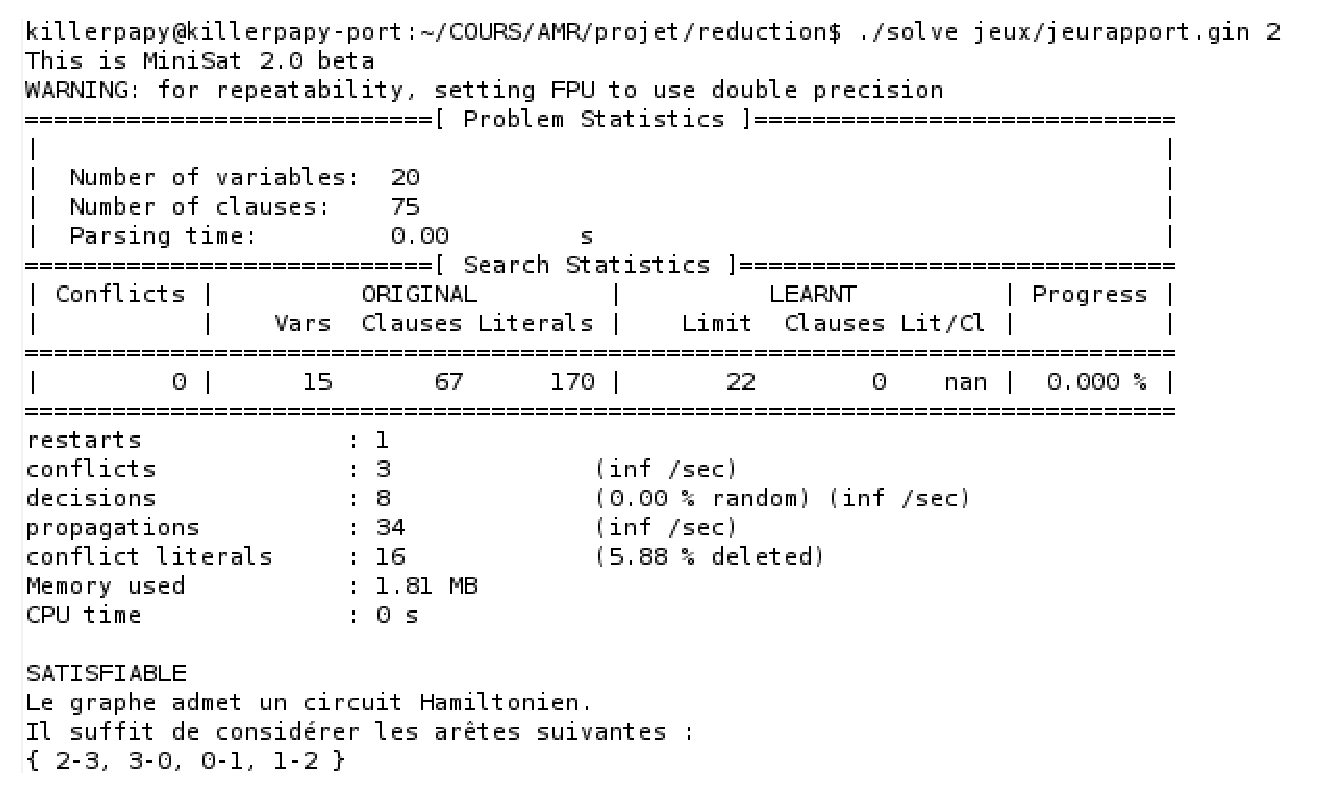
\includegraphics[width=12cm]{images/chemin.eps}
    \caption{\emph{Circuit Hamiltonien} sur le graphe
    \ref{graphe1}.\label{ham}}
   \end{center}
  \end{figure}
 \section{Bilan}
 
  \subsection{Difficultés rencontrées}
  Tout au long de notre projet, nous nous sommes heurtés à des
  difficultés.

  Nous avons eu quelques soucis de démarrage avec ce que l'on appelle
  communément la barrière du langage. En effet, n'ayant jamais créé un
  programme en \emph{C++}, les évidences, pour nous, n'en étaient
  pas. Les pointeurs que nous avions gentiment mis de côté dans notre
  esprit se sont rappelés à nous via des erreurs de
  compilation\footnote{Ce qui, vous en conviendrez, n'est pas la plus
  agréable façon de se retrouver.}. Cela nous a suivi tout au long de
  notre développement et continuera, à l'évidence, à nous suivre dans la
  suite du projet. 

  Au niveau des réductions, nous avons eu quelques problèmes, mais rien
  d'anormal. Nous avons de temps en temps oublié quelques propriétés
  mais nous nous en rendions assez rapidement compte en faisant tourner
  le programme sur des exemples.\\
  Néanmoins, \emph{Circuit Hamiltonien} nous a pris à revers dans la
  dernière ligne droite. En effet, nous n'avions pas considéré le cas du
  graphe formé de deux losanges rejoints par une arête (voir
  \ref{an_warningCH} page \pageref{an_warningCH} en annexe). Une refonte
  totale de notre réduction a dû être opérée car nous avions utilisé des
  variables sur les arêtes, ce qui n'éliminait pas le problème. C'est en
  nous inspirant de la réduction de \emph{Clique} à \emph{SAT} que nous
  avons refait celle pour \emph{Circuit Hamiltonien}.

  Nous avons eu aussi des problèmes au niveau de la concordance des
  différents emplois du temps qui fut pour nous
  \emph{NP-difficile}. Néanmoins ce problème n'était pas à l'insu de
  notre plein gré, car la composition du groupe ne nous était pas
  imposée.

  Dernier problème et non le moindre, la contrainte de temps et le
  chevauchement des projets. En effet, nous n'avons pas pu faire tout ce
  que nous aurions aimé réaliser. Nous allons donc vous donner quelques
  idées d'améliorations que nous avons eues mais que nous n'avons pas pu
  inclure dans notre programme.
  
  \subsection{Améliorations}
  Nous allons rapidement vous donner une courte liste des choses que
  nous aurions aimé mettre en place dans le projet mais n'ont pas pu
  l'être :
  \begin{enumerate}
   \item Vérifier les formats des fichiers en entrée\footnote{Nous avons
	 remarqué que si \emph{Solve.cpp} était un graphe, alors il
	 admettrait un \emph{Ensemble Indépendant} de taille $5$.} 
   \item Trouver plus de ``cas faciles''
   \item Donner le choix d'afficher ou pas l'exécution de
	 \emph{minisat}. Il faudrait gérer l'option -v qui, si elle
	 présente, permettrait d'afficher l'exécution de minisat, et
	 sinon, écrirait cette exécution dans \emph{graph.min} (il faut
	 utiliser une redirection de la sortie d'erreur de
	 \emph{minisat} ($2>$))
   \item Gérer les envois de signaux. Typiquement, durant l'exécution de
	 \emph{minisat}, si on fait un \emph{C-c}, le résultat affiché
	 est quelque peu effrayant
   \item Utiliser des structures de graphe différentes selon les
	 réductions
  \end{enumerate}
  
  \subsection{Conclusion}
  Tout d'abord, avant de conclure sur le travail effectué, nous tenons à
  exprimer le fait que nous sommes déçus de ne pas avoir pu expliquer
  plus en détail les raisonnements qui nous ont faits avancer dans le
  projet, notamment en ce qui concerne les réductions. Nous trouvons
  dommage que notre rapport doive se réduire à cinq
  pages\footnote{Rapport $\leq_P$ Cinq-pages}.

  Finalement, grâce au travail que nous avons effectué, nous avons
  compris l'utilité des réductions dans la pratique. Nous avons pu
  toucher du doigt la \emph{NP-complétude} et entrevoir les limites à la
  fois de nos réductions et du \emph{SAT-Solver Minisat}.
 \section{Annexes}
  \subsection{Test de couverture par sommets qui n'aboutit pas...\label{an1}}
  Couverture par sommets arrétée après plus de 15 minutes: image
  \ref{lourd} page \pageref{lourd}. Même après plus de 30 minutes le
  résultat est le même mais nous n'avons pas d'image pour celui-là car
  nous avons dû redemarrer le pc... En effet on voit la memoire se
  remplir jusqu'à être pleine.

  \begin{figure}[!ht]
   \begin{center}
    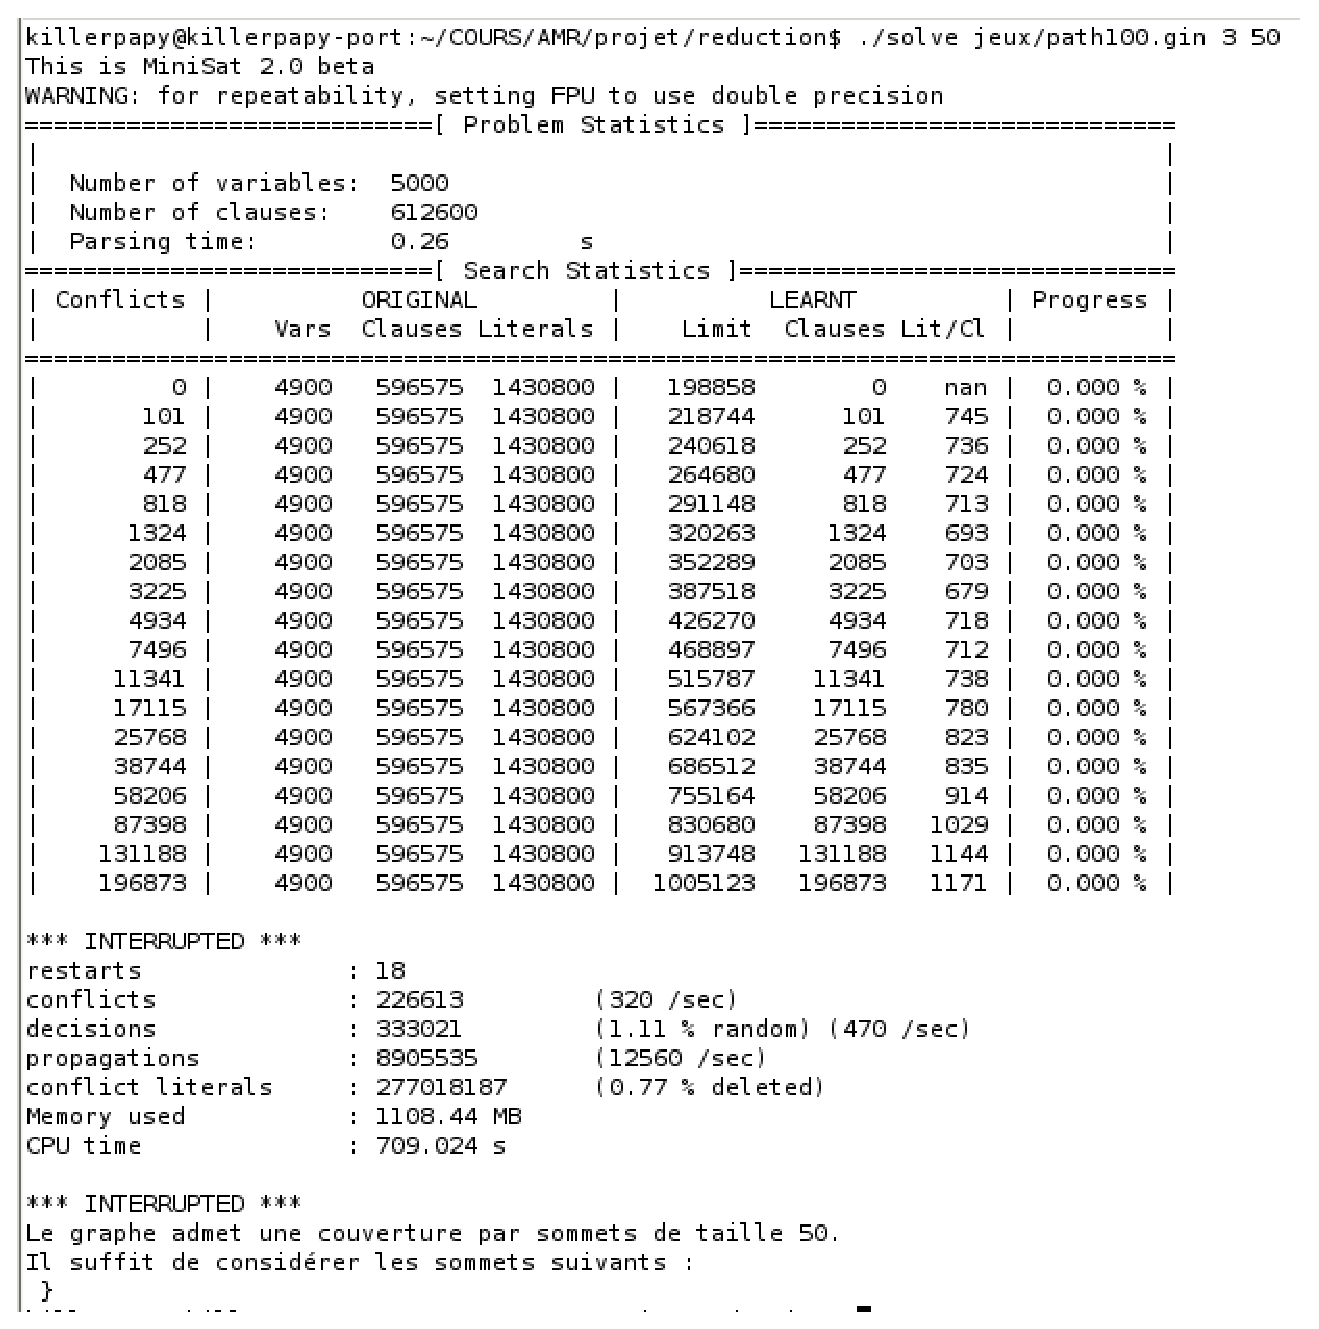
\includegraphics[width=12cm]{images/couv100.eps}
    \caption{\emph{Couverture par sommets} de taille 50 dans un chemin
    de taille 100.\label{lourd}}
   \end{center}
  \end{figure}

  \newpage

  \subsection{Test de K-Col sur un petit graphe\label{an2}}
  \emph{3-Col} sur graphe \ref{graphe} page \pageref{graphe} de petite
  taille.
  \begin{figure}[!ht]
   \begin{center}
    \includegraphics[height=6cm]{images/jeurap.ps}
    \caption{Exemple de graphe à 4 sommets.\label{graphe}}
   \end{center}
  \end{figure}
  
  \begin{figure}[!ht]
   \begin{center}
    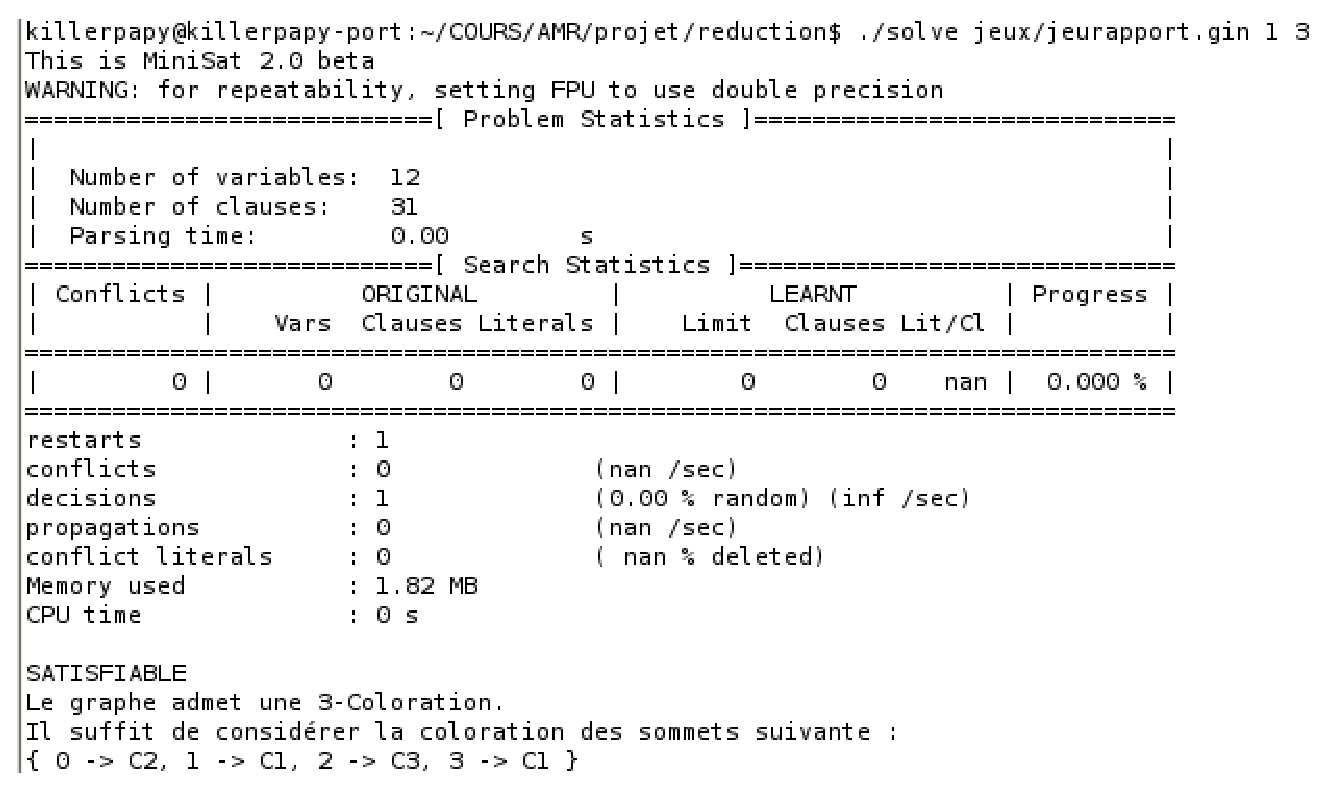
\includegraphics[width=12cm]{images/3-Col.eps}
    \caption{Test de 3-Col sur le graphe \ref{graphe}}
   \end{center}
  \end{figure}
  
  Ce qui donne comme résultat pour \emph{3-Col}: fig.\ref{result} page
  \pageref{result}
  \begin{figure}[!ht]
   \begin{center}
    \includegraphics[height=6cm]{images/jeurapport.ps}
    \caption{Test de 3-Col sur le graphe \ref{graphe} \label{result}}
   \end{center}
  \end{figure}

  \newpage

  \subsection{Circuit Hamiltonien - Cas dangereux\label{an_warningCH}}
  Cas dangereux de graphe qui n'admet pas de \emph{Circuit Hamiltonien}
  (fig.\ref{warningCH} page \pageref{warningCH}).
  \begin{figure}[!ht]
   \begin{center}
    \includegraphics[height=8cm]{images/warningCH.eps}
    \caption{Graphe dangereux pour \emph{Circuit
    Hamiltonien}\label{warningCH}}
   \end{center}
  \end{figure}





%%%%%%               %%%%%%
%%%%%% /ZONE DE CODE %%%%%%
%%%%%%               %%%%%%

\end{document}

%%%%%%           %%%%%%
%%%%%% /DOCUMENT %%%%%%
%%%%%%           %%%%%%




%%%%% Texte italique %%%%%
%  \textit{} 

%%%%% Liste %%%%
%%% Itemize %%%
%  \begin{itemize}
%   \item item1\\
%   \item item2
%  \end{itemize}

%%% Enumerate %%%
%  \begin{enumerate}
%   \item item1
%   \item item2
%  \end{enumerate}

%%%%% Tabulations %%%%%
%   \begin{tabbing}
%    XX\=XX\=\kill
%    \>(OrdresEnonce.v, ligne 244)\\
%    \>\>test2
%   \end{tabbing}
 
%%%%% Note de pied de page %%%%%
%  \footnote{test}

%%%%% Référence %%%%%
%   \label{ref}
%% Plus loin :
%   \ref{ref}
%   \pageref{ref}

%%%%% Code %%%%%
% \begin{lstlisting}
%      List<Integer> lexBFS2 = new ArrayList<Integer>();
%      lexBFS2.add(3);
%      lexBFS2.add(2);
%      lexBFS2.add(4);
%      lexBFS2.add(1);
%      lexBFS2.add(0);    
%      assertNotNull(lexBFS2);	
%      assertEquals(lexBFS2,Graphs.lexBFS(nogYComp));
%   \end{lstlisting}

%%%%% Figure %%%%%
%  \begin{figure}[!ht]
%   \begin{center}
%	\includegraphics[width=7cm]{figs/cours1/fig2.eps}
%	\caption{\emph{MT2} : Calcul non déterministe}
%   \end{center}
%  \end{figure}
